% UCL Thesis LaTeX Template
%  (c) Ian Kirker, 2014
% 
% This is a template/skeleton for PhD/MPhil/MRes theses.
%
% It uses a rather split-up file structure because this tends to
%  work well for large, complex documents.
% We suggest using one file per chapter, but you may wish to use more
%  or fewer separate files than that.
% We've also separated out various bits of configuration into their
%  own files, to keep everything neat.
% Note that the \input command just streams in whatever file you give
%  it, while the \include command adds a page break, and does some
%  extra organisation to make compilation faster. Note that you can't
%  use \include inside an \include-d file.
% We suggest using \input for settings and configuration files that
%  you always want to use, and \include for each section of content.
% If you do that, it also means you can use the \includeonly statement
%  to only compile up the section you're currently interested in.
% You might also want to put figures into their own files to be \input.

% For more information on \input and \include, see:
%  http://tex.stackexchange.com/questions/246/when-should-i-use-input-vs-include


% Formatting and binding rules for theses are here: 
%  https://www.ucl.ac.uk/students/exams-and-assessments/research-assessments/format-bind-and-submit-your-thesis-general-guidance

% This package goes first and foremost, because it checks all 
%  your syntax for mistakes and some old-fashioned LaTeX commands.
% Note that normally you should load your documentclass before 
%  packages, because some packages change behaviour based on
%  your document settings.
% Also, for those confused by the RequirePackage here vs usepackage
%  elsewhere, usepackage cannot be used before the documentclass
%  command, while RequirePackage can. That's the only functional
%  difference as far as I'm aware.
\RequirePackage[l2tabu, orthodox]{nag}


% ------ Main document class specification ------
% The draft option here prevents images being inserted,
%  and adds chunky black bars to boxes that are exceeding 
%  the page width (to show that they are).
% The oneside option can optionally be replaced by twoside if
%  you intend to print double-sided. Note that this is
%  *specifically permitted* by the UCL thesis formatting
%  guidelines.
%
% Valid options in terms of type are:
%  phd
%  mres
%  mphil
%\documentclass[12pt,phd,draft,a4paper,oneside]{ucl_thesis}
\documentclass[12pt,mphil,a4paper,oneside]{ucl_thesis}


% Package configuration:
%  LaTeX uses "packages" to add extra commands and features.
%  There are quite a few useful ones, so we've put them in a 
%   separate file.
% -------- Packages --------

% This package just gives you a quick way to dump in some sample text.
% You can remove it -- it's just here for the examples.
\usepackage{blindtext}

% This package means empty pages (pages with no text) won't get stuff
%  like chapter names at the top of the page. It's mostly cosmetic.
\usepackage{emptypage}

% The graphicx package adds the \includegraphics command,
%  which is your basic command for adding a picture.
\usepackage{graphicx}

% The float package improves LaTeX's handling of floats,
%  and also adds the option to *force* LaTeX to put the float
%  HERE, with the [H] option to the float environment.
\usepackage{float}

% The amsmath package enhances the various ways of including
%  maths, including adding the align environment for aligned
%  equations.
\usepackage{amsmath}

% Use these two packages together -- they define symbols
%  for e.g. units that you can use in both text and math mode.
\usepackage{gensymb}
\usepackage{textcomp}
% You may also want the units package for making little
%  fractions for unit specifications.
%\usepackage{units}


% The setspace package lets you use 1.5-sized or double line spacing.
\usepackage{setspace}
\setstretch{1.5}

% That just does body text -- if you want to expand *everything*,
%  including footnotes and tables, use this instead:
%\renewcommand{\baselinestretch}{1.5}


% PGFPlots is either a really clunky or really good way to add graphs
%  into your document, depending on your point of view.
% There's waaaaay too much information on using this to cover here,
%  so, you might want to start here:
%   http://pgfplots.sourceforge.net/
%  or here:
%   http://pgfplots.sourceforge.net/pgfplots.pdf
%\usepackage{pgfplots}
%\pgfplotsset{compat=1.3} % <- this fixed axis labels in the version I was using

% PGFPlotsTable can help you make tables a little more easily than
%  usual in LaTeX.
% If you're going to have to paste data in a lot, I'd suggest using it.
%  You might want to start with the manual, here:
%  http://pgfplots.sourceforge.net/pgfplotstable.pdf
%\usepackage{pgfplotstable}

% These settings are also recommended for using with pgfplotstable.
%\pgfplotstableset{
%	% these columns/<colname>/.style={<options>} things define a style
%	% which applies to <colname> only.
%	empty cells with={--}, % replace empty cells with '--'
%	every head row/.style={before row=\toprule,after row=\midrule},
%	every last row/.style={after row=\bottomrule}
%}


% The mhchem package provides chemistry formula typesetting commands
%  e.g. \ce{H2O}
%\usepackage[version=3]{mhchem}

% And the chemfig package gives a weird command for adding Lewis 
%  diagrams, for e.g. organic molecules
%\usepackage{chemfig}

% The linenumbers command from the lineno package adds line numbers
%  alongside your text that can be useful for discussing edits 
%  in drafts.
% Remove or comment out the command for proper versions.
%\usepackage[modulo]{lineno}
% \linenumbers 


% Alternatively, you can use the ifdraft package to let you add
%  commands that will only be used in draft versions
%\usepackage{ifdraft}

% For example, the following adds a watermark if the draft mode is on.
%\ifdraft{
%  \usepackage{draftwatermark}
%  \SetWatermarkText{\shortstack{\textsc{Draft Mode}\\ \strut \\ \strut \\ \strut}}
%  \SetWatermarkScale{0.5}
%  \SetWatermarkAngle{90}
%}


% The multirow package adds the option to make cells span 
%  rows in tables.
\usepackage{multirow}


% Subfig allows you to create figures within figures, to, for example,
%  make a single figure with 4 individually labeled and referenceable
%  sub-figures.
% It's quite fiddly to use, so check the documentation.
%\usepackage{subfig}

% The natbib package allows book-type citations commonly used in
%  longer works, and less commonly in science articles (IME).
% e.g. (Saucer et al., 1993) rather than [1]
% More details are here: http://merkel.zoneo.net/Latex/natbib.php
%\usepackage{natbib}

% The bibentry package (along with the \nobibliography* command)
%  allows putting full reference lines inline.
%  See: 
%   http://tex.stackexchange.com/questions/2905/how-can-i-list-references-from-bibtex-file-in-line-with-commentary
\usepackage{bibentry} 

% The isorot package allows you to put things sideways 
%  (or indeed, at any angle) on a page.
% This can be useful for wide graphs or other figures.
%\usepackage{isorot}

% The caption package adds more options for caption formatting.
% This set-up makes hanging labels, makes the caption text smaller
%  than the body text, and makes the label bold.
% Highly recommended.
\usepackage[format=hang,font=small,labelfont=bf]{caption}

% If you're getting into defining your own commands, you might want
%  to check out the etoolbox package -- it defines a few commands
%  that can make it easier to make commands robust.
\usepackage{etoolbox}

\usepackage{caption}
\usepackage{subcaption}

% Sets up links within your document, for e.g. contents page entries
%  and references, and also PDF metadata.
% You should edit this!
\input{LinksAndMetadata}

% And then some settings in separate files.
\input{FloatSettings} % For things like figures and tables
\bibliographystyle{ieeetr}   % For bibliographies

% These control how many number sections your subsections will take
%    e.g. Section 2.3.1.5.6.3
%  and how many of those will get put into the contents pages.
\setcounter{secnumdepth}{3}
\setcounter{tocdepth}{3}


\begin{document}

\nobibliography*
% ^-- This is a dumb trick that works with the bibentry package to let
%  you put bibliography entries whereever you like.
% I used this to put references to papers a chapter's work was 
%  published in at the end of that chapter.
% For more information, see: http://stefaanlippens.net/bibentry

% If you haven't finished making your full BibTex file yet, you
%  might find this useful -- it'll just replace all your
%  citations with little superscript notes.
% Uncomment to use.
%\renewcommand{\cite}[1]{\emph{\textsuperscript{[#1]}}}

% At last, content! Remember filenames are case-sensitive and 
%  *must not* include spaces.
% I may change the way this is done in a future version, 
%  but given that some people needed it, if you need a different degree title 
%  (e.g. Master of Science, Master in Science, Master of Arts, etc)
%  uncomment the following 3 lines and set as appropriate (this *has* to be before \maketitle)
% \makeatletter
% \renewcommand {\@degree@string} {Master of Things}
% \makeatother

\title{A Thesis Title}
\author{Thanh Trung Mai}
\department{Medical Physics and Biomedical Engineering}

\maketitle
\makedeclaration

\begin{abstract} % 300 word limit
My research is about stuff.

It begins with a study of some stuff, and then some other stuff and things.

There is a 300-word limit on your abstract.
\end{abstract}

\begin{impactstatement}

UCL theses now have to include an impact statement. \textit{(I think for REF reasons?)} The following text is the description from the guide linked from the formatting and submission website of what that involves. (Link to the guide: {\scriptsize \url{http://www.grad.ucl.ac.uk/essinfo/docs/Impact-Statement-Guidance-Notes-for-Research-Students-and-Supervisors.pdf}})

\begin{quote}
The statement should describe, in no more than 500 words, how the expertise, knowledge, analysis,
discovery or insight presented in your thesis could be put to a beneficial use. Consider benefits both
inside and outside academia and the ways in which these benefits could be brought about.

The benefits inside academia could be to the discipline and future scholarship, research methods or
methodology, the curriculum; they might be within your research area and potentially within other
research areas.

The benefits outside academia could occur to commercial activity, social enterprise, professional
practice, clinical use, public health, public policy design, public service delivery, laws, public
discourse, culture, the quality of the environment or quality of life.

The impact could occur locally, regionally, nationally or internationally, to individuals, communities or
organisations and could be immediate or occur incrementally, in the context of a broader field of
research, over many years, decades or longer.

Impact could be brought about through disseminating outputs (either in scholarly journals or
elsewhere such as specialist or mainstream media), education, public engagement, translational
research, commercial and social enterprise activity, engaging with public policy makers and public
service delivery practitioners, influencing ministers, collaborating with academics and non-academics
etc.

Further information including a searchable list of hundreds of examples of UCL impact outside of
academia please see \url{https://www.ucl.ac.uk/impact/}. For thousands more examples, please see
\url{http://results.ref.ac.uk/Results/SelectUoa}.
\end{quote}
\end{impactstatement}

\begin{acknowledgements}
Acknowledge all the things!
\end{acknowledgements}

\setcounter{tocdepth}{2} 
% Setting this higher means you get contents entries for
%  more minor section headers.

\tableofcontents
\listoffigures
\listoftables


\chapter{Introduction}
\label{chapterlabel1}

Computational models have been used in many research areas such as geology, physics or engineering to predict outcomes of complex problems. Computational models are usually constructed by applying an established physical principle that relate time-dependent variables which describe the state of the system to measured model parameters. This makes the models suitable to study the complex dynamic processes and system and predict the future behaviour of the system. In recent years, with the increase of computational power, fields such as biology or medicine, where the models can depend on a multitude of variables, have been using computational models as a framework to predict the behaviour of the systems and study the processes that are not fully understood.\par

In medical research, computational models have become a powerful tool to establish the fundamental understanding of the biology and anatomy in human body and also for medical device design. The consideration of using computational framework for diagnosis and interventional planning has been also gaining traction and numerous research areas have been emerged to create a tool that could assist the clinicians in their decision-making. One of these areas has been shown to be the the study of cardiovascular haemodynamics. \par

Over the past decade, the use of computational modelling in the cardiovascular research has showed numerous different approaches that could be benefitial for the clinical use. The use of computational models with patient-specific inputs can result in spatial and temporal data on parameters such as flow, velocity gradient, pressure, wall shear stress and vessel motion which could be used for decision making process. Additionally, the models can be parametrically modified to assist clinicians in investigating the outcome of various treatment methods.

Despite the numerous effort in making cardiovascular models viable for the clinical support, there are still numerous major challenges to these models viable in the use decision support. In fact, the choice of using computational models have been also dismissed due to these shortcomings. Often, patient-specific data in certain areas could be lacking thus simplifications of the real-life process would be necessary. Furthermore, due to the lack of data, often the models are run in an "idealized" scenario which can yield uncertain results. Lastly, there is a very little consensus in the cardiovascular modelling on the assessment of these uncertainties and variability.  \par
\chapter{Background}
\label{chapterlabel3}
In this chapter the basic background of the cardiovascular system and computational fluid dynamics will be introduced. Additionally, the process of verification, validation and uncertainty quantification will be explained.


\section{Cardiovascular system}
The cardiovascular system, also called the circulatory system, is a closed-loop system composed by the heart, blood vessels and blood. It uses blood as the medium to distribute oxygen and nutrients to all body tissues and dispose of carbon-dioxide and metabolic waste to lungs and excretory organs. Additionally, the secondary function of the system is to redistribute bioactive agents and hormones throughout the body, and regulate the body temperature \cite{Levick2010Introduction5ed}.\par

The heart is a muscular organ that  pumps the blood into the blood vessels to distribute it around the body. It is located in between the lungs above the sternum. The heart is divided into two sides and each side is divided further into two chambers (as seen on Figure \ref{fig:heart}. The top chambers are the atria and the bottom ones are the ventricles. The wall of the heart are composed of cardiac muscle which produce contraction that pump the blood into the arteries \cite{aaronson2012cardiovascular,tortora2017introduction}. \par

The system is divided into two circulatory loops with heart at the center, a pulmonary circulation and systemic circulation. In the pulmonary circulation, the deoxygenated blood is pumped from the heart's right ventricle into the pulmonary artery, where the blood is transported into the lungs where an oxygen exchange occurs. The blood then returns to the left atrium, passes through the left ventricle into the systematic circulation\cite{Levick2010Introduction5ed,tortora2017introduction}. \par


%The cardiovascular system is a closed-loop system composed of the heart, blood vessels and blood. The main function of the system is to distribute oxygen and other nutrients to all body tissues. Additionally, it also transports carbon-dioxide and other waste products to the lungs and excretory organs \cite{tortora2017introduction, aaronson2012cardiovascular}. The cardiovascular system has also a control function that redistributes hormones and bioactive agents and regulates the body temperature \cite{Levick2010Introduction5ed}.\par

\begin{figure}[ht!]
  \centering
  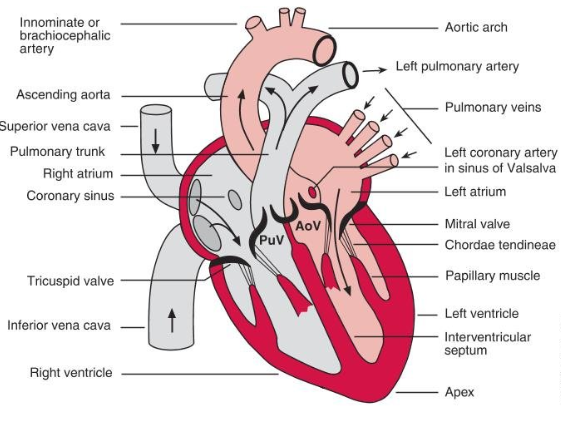
\includegraphics[width=0.6\textwidth]{Figures/heart}
  \caption{Structure of the heart and connection to the major veins and arteries \cite{Levick2010Introduction5ed}.}
  \label{fig:heart}
\end{figure}

%The driving force of the whole system is the heart, which is situated between the lungs behind the sternum above the diaphragm. The heart is divided into a right side and a left side by a layer called septum in between (as seen in Figure \ref{fig:heart}). Each of these sides is made up of two chambers, an atrium and a ventricle. The walls of the heart are composed of cardiac muscle, which generates the contraction and drives the blood flow in and out of the heart. The deoxygenated blood enters the right atrium through the vena cava which then enters the right ventricle through the tricuspid valve and subsequently exits the heart into the pulmonary artery. The blood is then transported to the lungs where an oxygen exchange occurs. The oxygenated blood is then transported back into the left atrium, through the mitral valve into the left ventricle where the blood exits the heart into the aorta \cite{aaronson2012cardiovascular,tortora2017introduction}.\par

The blood vessels of the system are responsible to deliver the blood into organs and tissue. The blood is driven into the aorta from there it flows into the major arteries, which then deliver blood to the major regions and organs. The arteries can further branch out and then they converge into veins which transport the blood back into the heart \cite{Levick2010Introduction5ed}.\par

\section{Computational Fluid Modelling for cardiovascular applications}
In the cardiovascular research, computational models have been often use to study the haemodynamics of the system. These were often used for hypothesis creation, mechanistic understanding, device evaluation or educational purposes. With better imaging modality and improved devices to obtain patient measurements, the concept of patient-specific models have been emerge and their capability of being used in diagnosis or predictive medicine was considered. Where the models are made tailored to the patient anatomy.\par

The cardiovascular models can be categorized by their dimension. Zero-dimensional (0D), or lumped parameter, models divide the system into individual components. The governing equations are ordinary differential equations. It can be made analogous to an electrical circuit where the physiological processes pressure, flow and volume are equivalent to to voltage, charge and current. 0D models assumes the velocity and pressure are uniformly distributed and are used to study the pressure waveforms, however they have limited accuracy to estimate the central aortic pressure \cite{Alimohammadi2015AorticUnderstanding}. However these model can be extended to include additional biochemical and biomechanical processes \cite{Hose2019CardiovascularNext}. \par

One dimensional models (1D) care used to describe vascular components in which distribution of quantities along the vessel axis have to be taken into consideration and are essential when wave effects are important. These models are represented using partial differential equations in time and one spatial dimension. These models are used to simulate pressure and flow waveforms at any point of the arterial network according to their distributed properties and recently, they have been also used to reconstruct central aortic pressure \cite{Zhou2019APressure, Hose2019CardiovascularNext}. \par 

Most common patient-specific em

\subsection{Governing equations}
Blood is usually described as a continuous and incompressible viscous-fluid. The governing equations of the flow are the Navier-Stokes equations (\ref{eq:n_s}) which describe the conservation of momentum of a fluid. Thus, the flow can be calculated in conjunction with the conservation of mass equation (\ref{eq:con} ):
\begin{equation}
\frac{\partial \rho}{\partial t}+\nabla \cdot (\rho U) = 0 \\
\label{eq:con}
\end{equation}
\begin{equation}
\frac{\partial (\rho U)}{\partial t}+\nabla \cdot (\rho U \times U) = -\nabla p + \nabla \cdot \tau + S_{M}
\label{eq:n_s}
\end{equation}
where, $p$ and $\tau$ are the pressure and stress tensor, respectively and $U$ is the velocity of the flow. The term $S_M$ refers for any momentum of external forces to the system. \par

\subsection{Patient-specific data}
In order to create image-based patient-specific haemodynamics models, it is necessary to obtain geometry and flow data. \par

Imaging techniques such a computed tomography (CT) can be used to obtain a number of image slices which would then be used to reconstruct the 3D model of the tissue and organs of the patient. The method  uses ionising radiation which benefits from high spatial resolution and high penetration depth. However, CT scanning often has limited sensitivity and also exposes the patient to radiation \cite{Saremi2015CoronaryCT}. An alternative method to obtain the geometry can be magnetic resonance imaging (MRI) which uses the principles of electromagnetism to capture the images. It yields the images based on the radiofrequency of the tissue, generated by the hydrogen atoms within the tissues. Using MRI, the patient is not exposed to radiation or contrast agents. However, in comparison with the CT images, the MRI has lower spatial resolution and it is much more time-consuming to acquire whole 3D stack of images \cite{Maurovich-Horvat2012DifferentiationHearts, Karmonik2008ComputationalRates}.\par

Other patient-specific data such as volumetric flow, pressure  or wall motion data has to be obtained in order to create accurate haemodynamic models. There are numerous ways how these can be obtained, both invasively and non-invasively. While invasive methods can provide accurate measurements through the application of different sensors, it is not desirable to use these techniques for diagnostic purposes. Several non-invasive imaging techniques can be employed. Doppler echocardiography or phase contrast (PC) MRI has shown to be a good method for obtaining flow measurements non-invasively \cite{Whitlock2015NoninvasiveAorta}. For the motion of the wall, the time-resolved images must be obtained; this can be done using electrocardiogram (ECG) coupled with CT or 4D MRI data for example \cite{Bonfanti2017ComputationalData,Alimohammadi2015AorticUnderstanding}.

\subsection{Modelling assumptions}

\subsubsection{Viscosity model}
The blood is a complex fluid composed of red and white blood cells and platelets in plasma.\par

While blood exhibits non-Newtonian properties, many of the haemodynamic models assume blood as a Newtonian fluid in large arteries. While the strain rates in these vessels are very low \cite{Fung1997BiomechanicsCirculation}, the Newtonian fluid does not take into account the shear-thinning properties of blood. By increasing the shear rate on the blood, the viscosity decreases (as seen in Figure \ref{fig:visc}) as a result of the disaggregation and the deformation of red blood cells \cite{Gijsen1999TheModel,Cho1991EffectsFlows}. Simple non-Newtonian models, such as Carreau-Yasuda or the Casson model, have been used to approximate the complex behaviour of the blood and to improve the study of the properties of the blood in vessels  \cite{Alimohammadi2015PredictingApproach}. \par

\begin{figure}[ht!]
\centering
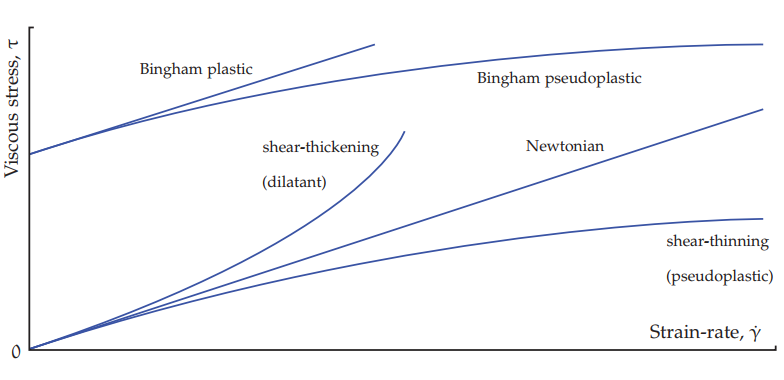
\includegraphics[width=\textwidth]{Figures/viscosity}
\caption{The relation of viscous stress and strain-rate, a comparison of Newtonian and non-Newtonian models \cite{Gabriel2017THEGROWTH}}
\label{fig:visc}
\end{figure}

\subsubsection{Flow models}
Another important consideration to take into account is the flow model which can be laminar, transitional or turbulent \cite{Morris2016ComputationalMedicine}. Turbulent flow introduces random fluctuations in the velocity resulting in turbulent eddies and dissipation of energy in the flow \cite{DongenF.N.vandeVosse2003CardiovascularMechanics}. The Reynold's number $Re$ which is the ratio of the inertial and viscous forces is used to determine the flow regime: 
\begin{equation}
Re = \frac{\rho UD}{\mu}
\end{equation}
Where D is the characteristic length, U is the velocity, $\rho$ is the density and $\mu$ is the viscosity.\par

In a flow, the transition to turbulence occurs at a critical ($Re_c$) of around 2000. The critical Reynold's number $Re$ can be determined using the Womersley number which is the ratio of transient inertial forces to viscous forces. However, it has been shown that in pulsatile flow that occurs in arteries, the $Re_c$ is much higher \cite{Alimohammadi2015PredictingApproach}.\par

A number of studies on the flow conditions in the arteries have found that $Re_c$ varies in the range 2700-15000 and that the maximum Reynolds number in arteries is up to 3700. Therefore, a majority of studies implement the flow as a laminar model. However, in more recent studies, it has been found, that transitional and turbulent regimes can occur in healthy ascending aortae and is more prevalent around aortic diseases \cite{Ku1997BLOODARTERIES}. \par




\section{Verification, validation and uncertainty quantification (VVUQ)}
While computational models can provide a framework to study the complex processes, it is necessary to question the credibility of computational models. The process of assessing models is done in three stages, verification, validation and uncertainty quantification (VVUQ), where different aspects of the models are evaluated. \par

Verification is the assessment of the mathematical and computational reliability. This can involve the assessment of the software quality, design and code review or the numerical analysis of the algorithm used in the code and it's properties (i.e. symmetry, stability, conservation, convergence, etc.). \par

The error of the model is evaluated by validation which compares the numerical results of the model with the true value obtained from the experiments. The process also involved the consideration of the uncertainty that stems from the experiments or from the simulation. 

\chapter{Literature review}
\label{chapterlabel3}

\section{Uncertainty}
In order to understand the effects of uncertainty on model prediction, it is important to know the different types of uncertainty and their source. In this section different  uncertainties will be explored.

\subsection{Sources of uncertainty}
There are numerous sources that can produce variability and errors. The different types of sources are shown below:
\begin{description}
\item[Residual variability] Variation due to the process being inherently unpredictable and stochastic. The latter can also be related to model inadequacy (structural uncertainty) due to the lack of details which eventually results in different process values. Usually to account for this variability, an average value is taken over these unrecognized condition to define the true values.
\item[Observational uncertainty] The two sources for this uncertainty stems from either limited or incomplete knowledge and measurement errors. The lack of knowledge can be a result of surrogates of the experiments or due to partial measurements. The measurements error is often attributed to the limited accuracy and resolutions of the sensors.
\item[Parameter uncertainty] The parameters of the model have to be specified in order to predict the behaviour of the process. The choice of the appropriate value of the parameters influences the process values as they can misrepresent the underlying physics.
\item[Condition uncertainty] In differential models, it is important to have initial and boundary conditions before the models is evaluated. These can be obtained from observations or experiments, thus, introduce uncertainties into the models.
\item[Structural (model) uncertainty] Also sometimes called model inadequacy. Models are a simplification of the real-world systems, therefore they are based on a certain number of more or less realistic hypothesis. In addition, some significant phenomena might have been neglected. The predicted values will not be equal to the true value of the process and the discrepancy between the two values is the structural uncertainty. 
\item[Simulator uncertainty] Computational results from a model is accompanied numerical errors associated with grid resolution, time steps,tolerances, convergence and any emulator approximations.
\end{description}

\subsection{Types of uncertainty}
Through identifying the sources of uncertainties, it is possible to classify the if the uncertainty could be reduced or not. The two types of uncertainties are:

\begin{description}
\item[Aleatory uncertainty] Also called statistical, stochastic or irreducible uncertainty, is the uncertainty due to the inherent variation and randomness that can occur in members of population due to spatial and temporal variations. These are typically unbiased and naturally defined using a probabilistic framework.
\item[Epistemic uncertainty] Uncertainty that arises due to simplification, assumptions or the lack of knowledge. Sometimes called reducible or ignorance uncertainty. The uncertainies are often biased and not often defined with a probabilistic network. However with additional knowledge, this uncertainty can be, in principle, eliminated.
\end{description}

\section{Uncertainty quantification methods}
There are several methods to assess the different types of uncertainties and quantify them in a probabilistic framework. In this section the different method of uncertainty quantification will be briefly explained.

\subsection{Input uncertainty}
Input uncertainty arises from uncertain inputs that are used for the model. These input that be either the observational data used in the model or parameter inputs that are determined to fit the model to the data. The uncertain input can be usually defined using a probability density function form the available information.\par

\paragraph{Monte-Carlo}
The Monte-Carlo (MC) algorithm is often used for uncertainty study due to its simplicity and wide-ranging applicability. The algorithm consist from three basic steps:
\begin{enumerate}
    \item A number of samples is drawn from a probability density function.
    \item For each of the drawn samples the model is evaluated.
    \item From the results calculated, the input uncertainty is determined.
\end{enumerate}
In order for the model to converge, a minimum number of samples has to be drawn which is however independent of the number of inputs. However it is important to note that the number of evaluations can be very high making it computationally expensive to run for certain models. 

\paragraph{Polynomial Chaos}
Another method to evaluate the uncertainty is using the polynomial chaos (PC) method. The method uses the polynomial expansion to decompose the model into polynomials. 

\subsection{Model uncertainty}
There are several methods that have been used in the field of computational modelling. The first two methods require a number of observations which are then compared with the model outputs. \par

\paragraph{Model Averaging}
The predictions or probability statements of a number of plausible models are averaged, with weights based either on some measure of model adequacy or some measure of the probability that the model is true. \par

Suppose there are a number of models present for a physical problems. Each model is evaluated using a model selection process, which can be either through Akaike's Information Criterion or Bayes' Information Criterion process. Instead of choosing a single best model, a number of best models are chosen and then a weight is applied and the model results are averaged. \par

\paragraph{Calibration-based methods } 
The focus of this method is on the model discrepancy $\mathbf{\delta} = \textbf{Z} - f(\textbf{X})$ , the discrepancy between the output of a model evaluated at the the true inputs and the true target value. The beliefs about $\mathbf{\delta}$ are updated based on the observations \textbf{Z} and the model is calibrated to minimize the discrepancy. \par

\paragraph{Internal discrepancy}
The model is divided into submodels, where the each submodels are evaluated individually using a method to determine the input uncertainty using one of the methods explained above. \par

The variation of each of submodel is then accounted in the whole model as additional parameter and the sensitivity of each parameter will be evaluated using the methods used to determine the input uncertainty. The parameter term that has the greatest impact on the model would be the most likely to the the most "uncertain". \par


\section{VVUQ in cardiovascular modelling}
In cardiovascular modelling, the process of verification and validation is often interchangable. Furthermore, often the validation process is comparing a single metric such as the outlet pressure or flow with the simulation. \par

While there are srict guidelines for the VVUQ of computational models and methods for UQ, they can be very mathematically very challenging and are often omitted from the analysis. Furthermore, in order to do an accurate analysis of the uncertainty, often a large number of $in vivo$ measurements if often necessary. \par

In the recent year, many of the researches also provide online dataset to establish a standardized dataset for the cardiovascular modelling community. Additionally, there have been also attempts to quantify the error and uncertainty. \par


\chapter{Aims and Objective}
\label{chapterlabel2}

In this report, the structural uncertainty due to the different modelling decisions will be explored. The appropriate metrics will be introduced and the areas that are most likely to introduce uncertainties will be addressed.\par

The following objectives will be investigated:
\begin{itemize}
    \item \textbf{Current work on uncertainty quantification from various fields:} Many fields that utilize computational models to predict systems behaviour have a framework to assess the uncertainties in the simulations. The different methodologies will be explored and reviewed on their suitability in their use in the framework of cardiovascular modelling.
    \item \textbf{Uncertainty and error quantification in cardiovascular engineering:} A literature review on the different studies of quantification of uncertainty and errors within the cardiovascular modelling community will be done.
    \item \textbf{Introduction of a systematic framework to address the different modelling assumptions made in cardiovascular models:} Through understanding of the different methods and reviews, a framework will be proposed on how to identify structural uncertainty and an example will be shown.
    \item \textbf{Identify the additional steps for the framework to be viable for uncertainty study:} This report will be a proof of concept that the framework would be an useful tool for studying the uncertainties in the cardiovascular models. In order to make the full framework, it is necessary to identify it's shortcomings.
\end{itemize}
\chapter{Methodology}
\label{chapterlabel5}
In order to identify the uncertain modelling assumptions, several models will be run. In this section, the process of evaluating the modelling assumption will be explained as well as the framework of assessing the uncertainties.

\section{Patient data}
The patient data was obtained from the Beijing Institute of Technology. The dataset included several geometries of patient's aorta and flowrate and luminal area waveform at the inlet and the outlets obtained via 4D-Flow MRI and cine-MRI. Additionally it also included the systolic and diasctolic measurement of the patiend and the heart rate of the patient as well. \par 

\section{0D model}
The whole system is initially described as a lumped model or also called the 0D model, where the different properties of the system are made analogous to electronics components. The model assumes that the parameters such as velocity and pressure are uniformly distributed. \par

\begin{figure}[ht!]
  \centering
  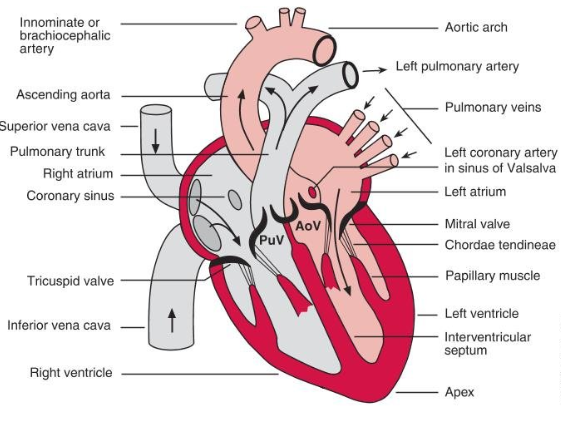
\includegraphics[draft]{Figures/heart}
  \caption{Schematic of the 0D model}
  \label{fig:0d}
\end{figure}

The aorta was divided in sections and which were represented with an elementary building block consisting of an inertance (L) and a resistance (R). The whole system can be seen on the Figure \ref{fig:0d}. The parameters of each section has been obtained from an steady state simulation CFD simulation, where the inlet was the average flow rate at the inlet measured from the 4D-MRI. The parameter were then calculated as:
\begin{align}
    L = \frac{\rho L}{A_{avg}}
\end{align}
\begin{align}
    R = \frac{\Delta P}{Q_{avg}}
\end{align}
where $\rho$ is the density, $L$ is the length of the segment, $A_{avg}$ is the average length of the section, $\Delta P$ is the pressure drop across the section and $Q_{avg}$ is the average flow rate at the section obtained from the patient's MRI dataset.\par

\begin{figure}[ht!]
  \centering
  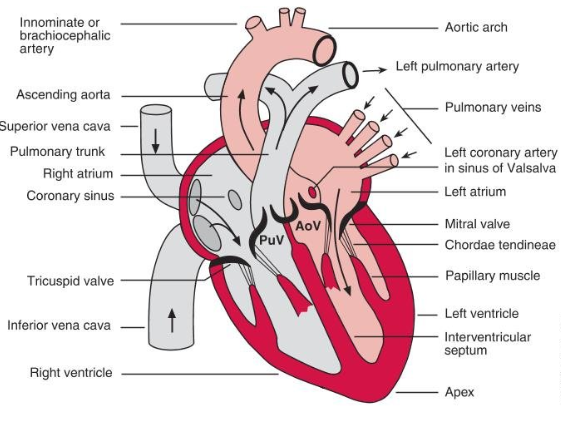
\includegraphics[draft]{Figures/heart}
  \caption{Windkessel models \textbf{a} two-element; \textbf{b} three-element; \textbf{c}} four-element
  \label{fig:wind}
\end{figure}

To account for the elasticity of at the outlet, an electronic analogous model will be used at the outlets, a Windkessel model (different types shown in Figure \ref{fig:wind}). The three-element Windkessel has been chosen for this study. While the two-element Windkessel is easier to implement, it cannot describe well the high frequency effects. The four element Windkessel can describe the impedance characteristics better, however due to the additional forth element, the parameters are difficult to estimate. Thus, the three-element Windkessel (WK3) model is often used theoretical research. \par

\subsection{Parameter tuning}
In order to get accurate parameters for the given pressure measurements and flow rates, an optimization algorithm was used. \par

Initially, the whole system is described as a single WK3 model where the $R_1$ and $R_2$ have been set as a ratio $R_1/(R_1+R_2) = 5.6\%$. Thus, only two parameters need to be fitted. The objective function minimizes the difference between the target systolic and diastolic pressure and the maximum and minimum pressure of the WK3 pressure curve which then gives:
\begin{align}
    min \sqrt{(P_{sys}-P_{max})^2+(P_{dia}-P_{min})^2}
\end{align}
 Additionally, non-negative constraints and bounding constraints have been applied for the parameters between the bounds [0, 2]. \par

Obtaining the parameters for the whole system, the compliance is distributed proportionally to $\bar{Q_i}$ to the outlets and the resistances are set as a ratio as seen previously. Therefore, for each of the outlet, only one parameter needs to be optimized. The objective function sums up the difference in the target and model pulse pressure and also the target and the model mean flow rate and for the parameters a non-negative constraints and bounding constraints as previously. Thus the objective function to be minimizes is as following:
\begin{align}
    min \sqrt{(P_{sys}-P_{max})^2+(P_{dia}-P_{min})^2+\sum_{i}(\bar{Q}_{i}^{target}-\bar{Q}_{i}^{0D})^2}
\end{align}


\section{Boundary conditions}
The blood is modelled as incompressible with a density 1060 $kg m^{-3}$ and the flow was considered as laminar, which is a common assumption in large arteries \cite{Alimohammadi2014DevelopmentConditions,Bonfanti2017ComputationalData}. The inlet condition was obtained from 4D-MRI and a flow rate was applied.\par

The three-element Windkessel parameters obtained from the 0D model has been coupled to the outlet, thus the mean pressure (P) and the flow (Q) at the outlet are related by:
\begin{align}
    P=(R_1+R_2)Q-R_2C\frac{dP}{dt}+R_1R_2C\frac{dQ}{dt}
\end{align}
where $R_1$, $R_2$ and $C$ are the parameters obtained for each of the outlet. \par

A no-slip condition was applied and the wall were considered as rigid. \par

\section{Modelling assumptions}
Different modelling assumptions can be used while modelling a patient aorta. The choice is often justified by the modeler but the resulting simulations can yield different results. In this section different modelling assumption that were taken into account are discussed and a number of combination of the assumption will be made resulting in 48 different CFD models.

\subsection{Segmentation}
While the patient geometries are obtained from the images, the segmentation criterion can affect the resulting in a varying geometry. While all geometry can be considered valid, this can results in differences in the lumen's area. \par

For the simulations, a two additional geometries will be used, where the patient's aorta is larger and narrower by 0.6 mm which accounts for the variability of the segmentation done (the original patient aorta was segmented from CT scans with 1 mm voxel). \par

\subsection{Image processing}
Depending on the image processing done on the patient scans the resulting geometry can have variation as well. These depend on the choices doing while improving the quality of the scans. \par

In the simulations two different aortas are being used, where one surface is smooth and the other is unsmoothened.

\subsection{Mesh}
While a finer mesh can yield much more accurate results, it comes with a trade-off of computational run time. In CFD simulatons it is a good practice to run mesh sensitivity studies before running the full simulation, however a proper guideline has not been introduced, therefore the decision on the mesh is often left to the modeler.\par

In this project a several meshes have been used to  assess how much the mesh can influence the final results. Four different meshes have been used with ~120,000 ~250,000, ~600,000, and ~1,100.000 elements.\par

\subsection{Viscosity}
As seen in the Chapter \ref{chapterlabel2}, while blood has shearing properties it is often assumed as Newtonian in larger arteries. Another approximation often used in simulations is using the Carreau-Yasuda model. \par

These two blood models will be considered, a Newtonian blood will be modelled with a constant viscosity of 0.004 $Pa s$ and the non-Newtonian blood will be modelled as Carreau-Yasuda model with the parameters taken from the Gijsen et al \cite{Gijsen1999TheModel}.


\section{Validation}
\chapter{Results}
\label{chapterlabel6}

One case from the permutations of the simulations is being used as the control model. The case was taken based on most common assumptions in the current research, which is the case of a normal aorta, smoothened wall and with Newtonian fluid. The mesh selected was the mesh 3(~ 600,000 elements).

\section{Outlet flow and pressure comparison}
A comparison of the outlet flow conditions were compared. As there was no patient data on the flow conditions apart from the flow rate, the percentage difference between the models has been calculated as:
\begin{align}
    \% diff = \frac{\bar{Q}_{mod1}-\bar{Q}_{mod2}}{\frac{\bar{Q}_{mod1}-\bar{Q}_{mod2}}{2}} \times 100 \%
\end{align}

A comparison of the different models show  that while the differences in pressures are very small, less then 1\%, the outlet flow can be result in very different results. \par

The most noticeable difference can be observed between the different segmentations of the patient aorta, where the mean difference of the flow at the outlet was 43.75\% followed by the image processing influence, where the difference was 34.05\%. The smallest difference was shown to be the influence of the viscosity model, as the difference across the outlets was smaller then 2\%. The influence of the mesh also showed to have very little effect on the outlet conditions where the flow rate differences were on average 2.64\%. \par

\section{Haemodynamic indices}


\chapter{Discussion}
\label{chapterlabel7}

In the results, the simulations of different model assumptions has been shown. The most significant differences can been seen on the model using unsmoothened aorta followed by the two geometries that were expanded and narrowed. While the unsmoothened geometry was still classified as "good", the differences can be seen on both the outlet condition and the haemodynamic indices. where the TAWSS values show to be much higher then in the other simulation. The choice of the image processing algorithm is often dependent on the decision taken by the modeler. Additionally due to the coupling of the 0D model to the 3D model, due to the varying area of the lumen, the Windkessel parameter tuned to the geometry would yield a different result in the 3D CFD simulation.\par

The modelling choices concerning images has shown to be a significant factor that influence the outcome of the CFD. In numerous CFD challenges, where the models were reconstructed from the images by a number of groupd, the image processing pipeline differed from group to group resulting in differences of TAWSS up to 40\% \cite{Steinman2018Editorial:Utility, Huberts2018WhatPaper}.\par

A comparison of the different blood modelling assumptions has shown very small differences between the models. The Newtonian fluid approximation is often widely accepted as the variation between the viscosity model are very minor, especially when compared with the effect of the image-based variations \cite{Steinman2019HowVariability, Lee2007OnBifurcation}. However in using a non-Newtonian blood can give important details on flow especially in the cases of smaller arteries and aneurysm studies \cite{Johnston2006Non-NewtonianSimulations, Steinman2012AssumptionsHemodynamics}. While there has been some studies of viscosity's influence on the blood flow in larger arteries, there is no objective reference that could quantify the variability therefore, the results were often interpreted subjectively \cite{Steinman2012AssumptionsHemodynamics}.\par

The different meshes in our simulations have produced very similar results. The study case in this project is relatively simple, however a more complex geometries would often require an appropriately sized mesh and a good quality. The meshes then vary from case to case therefore proper guidelines are difficult to provide. Furthermore, due to a number of different solvers, a numerical uncertainty factor is involved as well which is often hard to quantify as most of the CFD solver settings are hidden in the commercial software. \par
\chapter{Conclusion}
\label{chapterlabel8}
\chapter{Future Works}
\label{chapterlabel9}

While this project has to explored the different uncertainties that are involved in a CFD modelling of blood flow models, the study has been simplified as a proof of concept of the framework to identify the sources of biggest uncertainties in cardiovascular modelling. In this chapter the further work that will need to be done in order to create proper guidelines to use to the framework.

\section{Additional assumptions to consider}
In this project the image processing, segmentation, mesh size and the blood viscosity has been considered to quantify their effects on the simulation. However, there is a number of the other factors that can give rise to variability in the simulations.

\subsection{Rigid wall vs. Compliant wall}
While most of the CFD studies use the assumption that the walls are rigid wall, 
\phantomsection
\addcontentsline{toc}{chapter}{Appendices}

% The \appendix command resets the chapter counter, and changes the chapter numbering scheme to capital letters.
%\chapter{Appendices}
\appendix
\chapter{An Appendix About Stuff}
\label{appendixlabel1}

 % description of document, e.g. type faces, TeX used, TeXmaker, packages and things used for figures. Like a computational details section.
% e.g. http://tex.stackexchange.com/questions/63468/what-is-best-way-to-mention-that-a-document-has-been-typeset-with-tex#63503

% Side note:
%http://tex.stackexchange.com/questions/1319/showcase-of-beautiful-typography-done-in-tex-friends

% You could separate these out into different files if you have
%  particularly large appendices.

% Actually generates your bibliography. The fact that \include is 
% the last thing before this ensures that it is on a clear page.
\bibliography{references}

% All done. \o/
\end{document}
